\documentclass[man]{apa6}
\usepackage[square]{natbib}
\usepackage{microtype}
\usepackage{mathtools}
\usepackage{hyperref}
\usepackage{stmaryrd}
\usepackage{tabularx}
\usepackage[normalem]{ulem}
\linespread{1.3}
\hypersetup{colorlinks=true, citecolor=blue, urlcolor=red}
\shorttitle{disfluency/distraction}
\abstract{Where the veracity of a statement is in question, listeners show a bias towards interpreting speaker disfluency as a sign of dishonesty. 
This bias is not limited to post-hoc judgements, but can also be found during online speech processing. 
The present study investigates whether listeners are influenced by contextual information about the potential causes of speaker disfluency. 
If listeners make inferences about the cause of a disfluency, then a plausible speaker-distraction may attenuate the inclination to interpret an utterance as dishonest. \\

Participants listened to a speaker describe the locations of treasure (``The treasure is behind [the]/[thee---uh---] \textless referent\textgreater .''), while viewing scenes comprising the referent and a distractor. 
They were told that not all utterances would be honest, and their task was to click on the suspected location of the treasure. 
In line with previous work, participants were more likely to click on the distractor when the description was disfluent, and this effect corresponded to an early fixation bias, demonstrating the online nature of the pragmatic judgement.\\

The present study, however, also manipulated the presence of a plausible external cause of speaker disfluency. 
To accomplish this, participants were told that all utterances were produced outside on a busy street, and all items were played over low-level ambient street noise.\\

When there was a plausible external cause of the speaker disfluency (a distracting noise, in the form of a car-horn), participants were more likely to initially fixate on the referent, only later fixating on and selecting the distractor. 
One account of these findings would suggest that participants made early inferences about the contextual causes of disfluencies, which were eventually overridden by a dishonesty bias for disfluent utterances.}


\begin{document}
\title{Contextual effects on online pragmatic inferences.}
\author{JK; JL; MC}
\date{\today}
\maketitle

\section{Background.}
%\paragraph{intro, paralinguistic cues}
During conversation, rarely is an utterance or its delivery pre-planned.
Instead, everyday speech is for the most part spontaneous and thus often disfluent, containing pauses, ``um''s, ``uh''s, repetitions, revisions, and mispronunciations. 
Naturally occurring speech has a rate of approximately 6 to 10 disfluencies per 100 words \citep{Bortfeld2001, FoxTree1995}.
The disfluent nature of speech is just one of many variable aspects of \textit{how} an utterance might be presented, and listeners must be able to cope with this variability to successfully interpret a speaker.\\

These paralinguistic features of conversation are not merely incidental---often an utterance's manner of delivery is apposite to the message being conveyed, from the prosodic contour \citep{Fernald1991}, to an accompanying gesture \citep{Alibali2001}. 
In this way, numerous paralinguistic `cues' about the content of a speaker's message is readily available to listeners, and research has shown that listeners can, and do, exploit these phenomena \citep{Corley2007, Barr2001, Hostetter2011, Frazier2006}.
However, the way in which listeners interpret paralinguistic cues is not clear---do they simply rely on pre-learned direct associations of specific paralinguistic features with certain events in language, or do they use social and contextual information to draw inferences about why an utterance was produced in the way that it was? The latter suggestion would amount to a form a modelling the speaker's intentions, thoughts and perspective.\\

%\paragraph{disfluencies}
Disfluencies offer a listener cues about a speaker's planning processes, with rates of disfluency in speech increasing along with a speaker's cognitive load\citep{Bortfeld2001, Goldman-Eisler1968}.
Research shows that speakers are more disfluent when utterance planning involves low-frequency words \citep{Beattie1979}, less-preferred syntactic structures \citep{Cook2009}, discourse-new expressions \citep{Arnold2003}, and more choice of expressive alternatives \citep{Schachter1991}. 
Listeners, in turn, appear to associate speaker-disfluency with aspects of language which are perceived as more difficult to plan, displaying biases towards less predictable continuations \citep{Corley2007}, discourse-new referents \citep{Barr2001, Arnold2004}, and unfamiliar objects \citep{Arnold2007}.\\

The sensitivity which listeners display to the manner of an utterance's delivery facilitates the processes involved in comprehension of the linguistic message by generating expectations about upcoming speech. 
However, listeners' biases to disfluencies are not restricted to their predictions about the linguistic message, and also extend to global pragmatic judgments made about an utterance, such as estimates of the speaker's metacognitive state.
Utterances which are hesitant, disfluent, or with rising intonation are judged as less confident \citep{Smith1993, Brennan1995}.
This effect has shown to be present in various contexts---in both speaker's own and a listener's assessment of certainty \citep{Swerts2005}, and for both adult and child listeners \citep{Krahmer2005}.\\

When a speaker lies, however, we might perceive their utterance planning as more effortful, in order to convincingly convey a statement which they do not regard to be true.
Speaker-disfluency in particular, and especially pauses, appears to be frequently associated with an interpretation of dishonesty, in judgments made about speakers themselves as well as judgments made about other speakers \citep{Zuckerman1981}.
Research has shown that accuracy in discriminating truth from lies increases when presented with audio or audiovisual information rather than visual information \citep{Bond2006}, supporting the salience of vocal cues in recognising deception.\\

The effect of disfluency on listeners' pragmatic judgments about an utterance have, until recently, used offline measures of judgement (post-hoc assessment of a speaker's confidence or honesty). 
However, recent research has found that the disfluency-dishonesty bias is apparent from the early stages of reference comprehension. 
In a recent study by \citet{Loy2016}, subjects engaged in what was posed as a 'lie detection game', in which listeners were tasked to make implicit judgments about whether a speaker is being deceitful or not in indicating the location of a reward.
Utterances were presented as either fluent or disfluent (``The treasure is behind [the]/[thee---uh---] \textless referent\textgreater .''). 
In a visual world paradigm, listeners signalled their assessment of a speaker's honesty by clicking on one of two objects (the referent and a distractor) - interpreting an utterance as honest would result in a click on the referent, and as dishonest a click on the distractor.
In this way, \citet{Loy2016} investigated how listeners' pragmatic inferences about a speaker's honesty during online processing of speech was influenced by speaker-(dis)fluency.\\

\citet{Loy2016} found that, as with the influence of disfluencies on listeners' predictions about semantic content \citep{Arnold2004, Arnold2007, Barr2001}, manner of delivery's influence on listeners' pragmatic hypotheses emerges rapidly during the initial stages of refernce comprehension. 
Subjects' eye- and mouse-movements displayed a bias toward the referred-to object for fluent utterances, and to the distractor object for disfluent utterances \citep{Loy2016}.
This dishonesty-bias listeners' display to speaker-disfluency shows evidence of an ability to integrate information about utterance delivery and alter the global interpretation of an utterance during the moment-to-moment processing of speech.\\

The aforementioned studies give strong evidence for listeners having biases towards speaker-disfluency in terms of both semantic content \citep{Arnold2004, Barr2001} and pragmatic judgments \citep{Loy2016}, and for the emergence of these biases during the initial stages of the comprehension process.
The mechanism by which disfluency influences listeners interpretations, however, remains less clear. 
The disfluency-biases discussed above can all be explained in terms of a low-level account in which listeners' interpretations of disfluencies result from a prelearned stochastic model of co-occurrences of disfluencies with certain properties of language use. 
Listeners' bias towards associating presence of disfluency with discourse-new information could be due to distributional learning of disfluencies more often occurring when speakers refer to something new than to something familiar \citep{Arnold2004, Barr2001}. 
Likewise the disfluency-dishonesty bias in \citet{Loy2016} could result from a prelearned association \textcolor{red}{(or belief of an association)?} between disfluency and deception.\\

An alternative account suggests that speaker-disfluency is a form of collateral communication \citep{Clark1996}. 
As opposed to holding direct associations of disfluencies with language use, this view suggests that listeners interpret disfluency as communicative signals which manage discourse, and generate expectations by drawing inferences about its cause---e.g. about what might cause increased cognitive load for the speaker. 
This `disfluency-attribution' view is paired with the suggestion that speakers' production of fillers is akin to the use of conventional words, carrying a fundamental meaning of delay to which the listener can then attribute a cause \citep{Clark2002}. 
For the disfluency-deception bias, this account suggests that listeners interpreted disfluency by drawing an inference that e.g. the speaker's decision to lie resulted in more effortful utterance planning, thus causing disfluency.\\

Understanding the mechanisms underlying listeners' processing of disfluencies has wider implications for language comprehension in general. 
If listeners inferentially attribute cause to disfluency during online speech processing, this suggests that listener rapidly access information about what might cause delay for that particular speaker in that particular context. 
As such, this account implies that listeners engage in a form of modelling of the speaker.
In comprehension, accounting for a speaker's perspective has been argued to be costly in effort \citep{Lin2010}, as it requires continually accessing speaker- and context-specific information. 
Instead, many have suggested that listeners rely on less cognitively demanding, `egocentric' tactics, in which language is interpreted relevant to a listener's own perspective (or a minimally adapted version), and taking a speaker's perspective occurs only when entirely necessary \citep{Barr2002, Barr2004, Barr2014, Pickering2004, Kronmuller2007}.
If listeners' interpretations of disfluencies are moderated by speaker- and context-specific information, this suggests that the effect of disfluencies on comprehension cannot be the result of prelearned associations alone.
Instead, it would suggest that comprehension of disfluent speech involves taking into account what might lead a particular speaker to produce an utterance in a particular way, and as such, implies a form of perspective-taking.\\

%\paragraph{heller, barr, arnold}
Recently, several studies have provided evidence for disfluency-comprehension being context-dependent by examining how listeners' biases to disfluencies change when presented with alternative plausible causes of speaker-disfluency. 
\citet{Arnold2007} showed that a bias towards unfamiliar, hard-to-describe objects following a disfluency is moderated by listeners' beliefs about that speaker. 
The results of both a gating task and an eye-tracking task showed that a) the discourse-new bias found in \citet{Arnold2004} could be extended to an unfamiliarity-bias, and b) this bias was reduced when the listener believed the speaker to have object-agnosia (inability to recognize objects). 
Similarly, \citet{Barr2010} found that the discourse-new bias to disfluencies was dependent upon what was new for the speaker independent of what was new for the listener.
\citet{Heller2015} suggest that listeners use context-specific inferences about what objects may cause production delay---they found that listeners' bias towards unfamiliar objects adapted to novel contexts with artificial lexicons in which all objects were, to varying degrees, `unfamiliar'.\\

Whilst these studies show that listeners' disfluency-biases display a flexibility to speaker- and context-specific information, the extent to which listeners are engaging in inferential processing about causes of disfluency is disputable. 
For listeners' perceptions about the cause of disfluency, belief that the speaker is object-agnosic provides an utterance-global explanation for speaker-disfluency (familiar and unfamiliar objects being equally difficult to describe for an object-agnosic speaker). 
In this respect, whilst the integration of information evident in \citet{Arnold2007}, \citet{Barr2001}, and \citet{Heller2015} clearly requires some form of inferencing about the speaker or context, it is possible that listeners only engaged in the inferential process prior to speech onset. 
This could equate to essentially readjusting prior associations of disfluency and unfamiliar objects, rather than repeatedly making inferential judgments about cause of disfluency as speech unfolds.\\

To investigate whether listeners access context-specific information to engage in disfluency-attribution \textit{during} the online processing of speech, we ask whether listeners' disfluency-biases are flexible with regard to the presence of an utterance-local cause of speaker-disfluency---i.e. an explanation of disfluency which only presents itself \textit{during} the time-course of an utterance. 
Specficially, we look at whether listeners' pragmatic biases to disfluencies signalling deception \citep{Loy2016} is moderated by the availability of `speaker-distraction' as a cause of disfluency.\\

The current study develops \citet{Loy2016}'s visual world paradigm, with the addition of manipulating the presence of a disruptive (and so plausibly distracting) noise in the speaker's environment.
To accomplish this, subjects participated in the same `lie-detection task', but this time utterances were presented to listeners under the guise of having been recorded outside in a busy street.
Low-level ambient noise was present behind every utterance, and the potentially distracting noise took the form of a car-horn. 

The idea is that if utterance-local contextual information informs the online pragmatic judgments made about disfluency, this would suggest that listeners' inferential processing in attributing a cause to a disfluency is a) flexible, and b) occurs during the moment-to-moment processing of speech. 


Recording eye- and mouse- movements, we look at how the time course of pragmatic inferencing about speaker's disfluent message is influenced by the availability of an alternative, utterance-local cause of disfluency.
%mention traffic noise etc, car horn. 



\section{Method.}
\subsection{Materials.}
%\subsubsection{visual}
Visual stimuli consisting of 120 black and white line drawings, taken from \citet{Snodgrass1980}, were presented to participants in pairs across 60 trials (20 experimental, 40 fillers). 
Each trial presented the \textit{referent} (the object which the speaker identified as having the treasure behind for that trial), and a \textit{distractor}, which was chosen at random without replacement from a set of 60 objects. 
To control for the effect of the bias towards interpreting disfluency to difficulty of description \citep{Arnold2007}, critical referents and distractors were matched for familiarity (H value $\ge 3.0$) and ease-of-naming ($<1.0$). 
Object pairings with the same phonetic onset were avoided. \\

%\subsubsection{utterances/audio}
As in \citet{Loy2016} each referent was associated with a recording of a speaker naming the depicted object as the location of the treasure, and as before, critical utterances were either fluent or disfluent. 
The present study, however, manipulated not only the manner of delivery, but also the presence of a plausible cause of speaker distraction. 
Thus audio files were constructed such that the critical referents could be heard in four conditions in a 2 (fluent/disfluent) x 2 (distraction absent/present) design, see below. 
The insertion of a prolonged article followed by a filled pause into the fluent utterance formed the disfluent variants\footnote{We opted for utterance-medial disfluencies rather than utterance-initial as these sounded more believable as being caused by speaker distraction when paired with a environmental cue.}. 
%not footnote, put in main text
Meanwhile, to create a plausible cause of speaker-distraction, a 520ms car-horn sound effect was presented prior to the onset of the referent noun (-1100ms for disfluent utterances, -600ms for fluent). 
\begin{enumerate}
\item \textbf{fluent, distraction absent:} The treasure is behind the \textless referent\textgreater .
\item \textbf{disfluent, distraction absent:} The treasure is behind thee, uh ... \textless referent\textgreater .
\item \textbf{fluent, distraction present:} The treasure is $\underbracket{\text{behind the}}_\text{horn}$ \textless referent\textgreater .
\item \textbf{disfluent, distraction present:} The treasure is $\underbracket{\text{behind thee}}_\text{horn}$, uh ...\textless referent\textgreater .
\end{enumerate}

To situate the car-horn sound effect in a context, all recordings were presented overlaid upon a clip of ambient traffic and street noise which was unique to each referent. 
Thus the presentation of each critical referent varied only by 1) fluency and 2) presence of car-horn, to ensure that participants' behaviour was a reaction to the different combinations of these elements. 
All recordings, ambient noise and sound-effects were normalised and resampled to create 48 KHz stereo .wav files.\\
%This is confusing to me - does this mean that the audio stimuli for every trial lasted for 5000ms, regardless of utterance length? Wouldn’t there have been quite a bit of ambient traffic noise post-utterance if so? (And wouldn’t the post-utterance noise duration have varied quite a bit too? Or was this normalised by varying the pre-utterance amount of noise or something?) Sorry if I’m just being a bit thick.
%so, there was an amount of post-utterance noise (until mouse click), but for each referent, this noise was the same across conditions. 

%\subsubsection{lists}
The 20 critical items/referents were counterbalanced across four lists, each with 10 fluent and 10 disfluent utterances, and each containing 10 instances of the car-horn (5 of which were disfluent). 
Lists also contained 40 filler utterances, half of which were fluent, and half of which contained either a form of disfluency or a discourse manipulation (see Table \ref{table:fillers}). 
Additionally, 20 of these filler items (10 fluent, 10 disfluent/discourse manipulation) contained various novel noises which could be interpreted as distracting for a speaker (see Table \ref{table:fillernoise}). 
These filler distractions varied in position relative to the referent noun onset. \\

\subsection{Cover story.}
Central to the idea of a distraction-caused-disfluency is the requirement that participants believe that the utterances were produced naturally and in a noisy environment. 
Participants were told that the recordings were made by a participant of a previous experiment which was conducted on the side of a busy street. 
To corroborate this, during the initial explanation of the experiment, participants were shown three videos claimed to be examples of the speaker producing the utterances. 
These were presented alongside the images about which the speaker spoke. 
Speaker utterances were depicted in the first video as honest \& fluent, dishonest \& disfluent in the second, and, in the third, honest \& disfluent but distracted (speaker glances sideways toward a car following the car-horn sound effect).\\
%need more detail. - screen shot of video?

To ensure that analysis could be run only on data from participants for whom the cover story held, a post-test questionnaire assessed whether participants thought it believable that the utterances were produced naturally and in the suggested context. 
This was double-checked by verbal questioning after participants were debriefed about the true nature of the experiment, by asking whether it occurred to them during the experiment that the recordings might not have been produced outside in the street.\\

\subsection{Procedure.}
Stimuli were displayed on a 21'' CRT monitor, placed 850mm from an Eyelink 1000 Tower-mounted eye-tracker which tracked eye-movements at 500Hz (right-eye only). 
Audio was presented in stereo from speakers either side of the monitor. 
Mouse coordinates were sampled at 50Hz. 
The experiment was presented using OpenSesame version 3.0 \citep{Mathot2012}.\\

%\subsubsection{trial structure}
Participants were told they would see two objects and hear a speaker identify one of them as hiding the treasure. 
They were told that the objective of the game was to accrue treasure by successfully locating the treasure, the location of which the speaker would lie half the time about. Participants' instructions were to click on the object which \textit{they believed} the treasure to be behind. 
Once participants had read the instructions, the eye-tracker was calibrated.
Calibration was monitored throughout, with the experiment being paused for recalibration if the experimenter deemed it necessary.
To maintain accuracy, between each trial participants underwent a drift correction using a central fixation point, which changed from grey to red (for 500ms) upon successful fixation, signifying the start of the subsequent trial. 
Each trial began with the presentation of the two images (referent and distractor) in positions vertically central and horizontally to the left and right of centre (referents were presented equally often on each side). 
Simultaneous with presentation of the visual display was the onset of the ambient traffic audio file. 
After 1500ms, the mouse pointer appeared centrally, and the playback of the utterance began. 
Upon clicking an object, the stimuli disappeared and were replaced by the grey fixation dot, signifying progression to the subsequent trial. 
Each trial had an automatic time-out of 5000ms from utterance onset, in case participants did not click on an object.\\

%\subsubsection{bonus rounds}
To maintain motivation throughout the study, participants were told that there were a number of ``hidden bonus rounds'' which offered more treasure. 
Of the filler trials, 25\% did not immediately progress to the subsequent trial, instead giving a positive feedback message (regardless of which object was clicked) stating successful completion of a bonus round. 
Furthermore, participants were told that top scorers of the game would be able to enter their name on a highscore table, which was shown at the beginning of the experiment. 
Participants completed five practice trials (one of which was presented as a bonus round) prior to the main experiment. 
Eye-movements, mouse co-ordinates and object-clicked (referent/distractor) were recorded for each experimental trial.\\

\section{Results.}
\subsection{Exclusion criteria.}
For a final sample of 24, we were required to run the experient with 37 participants, recruited from the University of Edinburgh community, who participated in return for £4 remuneration. 
The data from 12 participants was excluded on the basis that they indicated either in the questionnaire (ten) or verbally (two) that they did not believe the cover story. 
Additionally, the study reported that one participant for whom the deception held had previously participated in \citet{Loy2016}, and thus they were also exlcuded. 
Analysis was run on the data from the remaining 24 participants.\\

\subsection{Analysis.}
Analysis was carried out in R version 3.3.0 \citep{rbase}, using the lme4 package \citep{lme4}. 
Trials in which participants did not click on either the referent or distractor (0.01\%) were excluded from all analyses. 
Object-clicked (referent/distractor) was modelled using mixed effect logistic regression, testing for main effects of manner of delivery, presence of plausible speaker distraction, and their interaction as fixed effects, and including random slopes for these same variables, plus random intercepts and slopes by both subject and referent. \\

Eye-tracking fixation data was averaged into 20ms bins (of 10 samples) prior to analysis, and coded in terms of the area of interest (AOI), which were referent; distractor and neither image. 
The proportion of fixations to either object from the total sum of fixations was computed for each time bin. 
Mouse-tracking analysis only looked at the x-coordinates of the cursor. Distance traveled by the cursor (pixels) was computed for each 20ms bin, coded for direction relative to either object. 
The cumulative mouse distance traveled toward either object in each trial was calculated by summing the distance travelled up to each time bin, and proportion of movement was calculated by taking the distance travelled toward an object, divided by the total distance travelled in that trial in either direction. 
Trials for which the total mouse distance travelled post referent-onset was less than 1/3 of the distance from the screen centre to the near edge of an object were excluded (0.03\% of trials), on the basis that it was indicative of participants' having decided prior to referent-onset upon which object to click. 
Movements beyond the outer edge of either object were excluded on the basis that it indicated `overshooting' with the cursor.\\

Model analysis for both eye- and mouse-movements were conducted over a time window from referent onset to 800ms post-onset. 
This window coincides with \citet{Loy2016}, identified by evidence that reference is established in eye-movements around the 400-800ms post noun-onset mark \citep{Eberhard1995}, and covering the duration of the longest critical referent (776ms). 
Models were estimated using empirical logit regression \citep{Barr2008} with main effects of time (scaled), object (referent/distractor), delivery (fluent/disfluent) and speaker distraction (absent/present), and interactions between them all, along with by-subject and by-item random intercepts and random slopes for time. \\

\subsection{Final object-click.}
Responses show the same overall tendency to interpret an utterance as truthful as was found in \citet{Loy2016}, with 57\% of trials resulting in a click on the referent and only 43\% on the distractor. 
Participants were less likely to click on the referent following a disfluent utterance than a fluent one ($\beta = -2.24,SE = 0.67,p<.001.$). 
This is in keeping with literature \citep{Brennan1995, Swerts2005} and with the results of \citet{Loy2016} - manner of delivery influences participants' global interpretation of the speaker's truthfulness. 
The presence of a plausible speaker distraction was not found to affect responses, neither was the interaction between delivery and distraction. 
The bias toward interpreting disfluency as a sign of dishonesty appeared to be explicit for 19/24 participants, as indicated in the post-test questionnaire. 
Table \ref{table:objctclck} shows the percentage of mouse-clicks on each object by condition.\\

\subsection{Eye-movements.}

The time-course (referent onset to 2000ms post-onset) of fixations to referent and distractor can be seen for the fluent conditions (Fig. \ref{fig:flueye}) and the disfluent conditions (Fig. \ref{fig:diseye}). 
Visualisation of the time-course of fixations show that for fluent utterances, participants displayed an early fixation bias towards the referent, which began to present itself prior to mean critical noun offset. 
For disfluent utterances, the picture is more complex---whilst a fixation bias towards the distractor was present, it appeared later on in the trial, not during the utterance of the critical noun as it did in \citet{Loy2016}. 
Although the same is true of utterances in which there was an available cause of speaker-disfluency, in these cases, participants appeared to fixate more to the referent first, before the later bias towards the distractor.\\

Model analysis of the window from referent-onset to 800ms post-onset confirmed what is evident from visualising the time-course of fixations. 
When presented with a fluent utterance, participants' fixations to the distractor decreased over time in favour of the referent ($\beta = -0.63, SE = 0.03, t=-18.51.$). 
In contrast, fixations to the distractor over the referent increased over time when the delivery was disfluent ($\beta = 0.59, SE = 0.05, t=12.24.$). 
When a plausible cause of speaker distraction was present, participants' fixation biases towards the distractor during disfluent utterances were reduced ($\beta = -0.20, SE = 0.07, t=-2.9.$). 
The presence of the speaker-distraction was not found to have an effect on the tendency to fixate on the referent for fluent utterances ($t=-0.9.$).\\

\subsection{Mouse-movements.}
The proportion of mouse movements (distance traveled) towards either object was computed for each 20ms bin from referent onset to 2000ms post-onset. 
Figures \ref{fig:mflu} and \ref{fig:mdis} and show the proportion of mouse movements towards either object in fluent and disfluent conditions respectively. 
Model analysis of the window from referent-onset to 800ms post-onset patterned with the eye-tracking data. 
When presented with a fluent utterance, participants' movements to the distractor decreased over time in favour of the referent ($\beta = -0.46, SE = 0.02, t=-19.49.$), whereas movements to the distractor over the referent increased over time when the delivery was disfluent ($\beta = 0.60, SE = 0.03, t=17.72.$). 
When a plausible cause of speaker distraction was present, participants bias towards moving to the distractor during disfluent utterances was reduced ($\beta = -0.35, SE = 0.05, t=-7.25.$).\\


\section{Discussion.}

Evidence of listeners' pragmatic judgments about a speaker's honesty based on manner of delivery emerged at an early stage in utterance processing, with eye- and mouse-tracking data showing biases towards referent and distractor for fluent and disfluent utterances respectively during the initial stage of the comprehension process. 
In this respect, the present study successfully replicates the effect found by \citet{Loy2016}, showing that an utterance's delivery influences listeners' pragmatic inferences about speaker's intentions to be (dis)honest. 
Additionally, the results here show that this effect is robust against the presentation of speech in a noisy environment, in which there are potential distractions for the listener. 
%More broadly, it goes some way to strengthening the ecological validity of the visual world paradigm - one could imagine a real world equivalent in terms of the sleight-of-hand 'thimblerig' game, in which spectators are asked to guess which of three containers an object is under, after they have seen it placed under one, and then watched their order be shuffled (stereotypically performed as a confidence trick on the street).
\\

The interest in this study, however, is in how listeners responded when presented with two competing explanations for the cause of speaker-disfluency. 
When an alternative explanation for speaker-disfluency was available to listeners, although the disfluency-dishonesty bias persisted in the final interpretation of an utterance (as evidenced by the eventual decision of which object to click), the picture during the initial stages of comprehension is more complex. 
The increase in fixations and mouse-movements to the distractor for disfluent conditions which occurred - indicating the emergent bias towards interpreting the utterance as dishonest - was initially attenuated when a possible cause of speaker-distraction was present. 
The availability of an external cause of the speaker disfluency resulted in a tendency to initially fixate and move toward the referent, only later fixating on and selecting the distractor. \\

One account of these findings would suggest that participants made early inferences about the contextual causes of disfluencies, which were eventually overridden by a dishonesty bias for disfluent utterances. 
By this account, listeners appear able to dynamically decide upon the most likely explanation of disfluency, and, as the speech unfolds, make attributions about why a speaker was disfluent. 
This equates to listeners engaging in a form of speaker/situation-modelling, in which judgments are made about a speaker's perspective and thought-processes. 
These judgments are then used to constrain the interpretation of the speaker's meaning\textsubscript{nn} and intentions. 
This evidence for perspective-taking in the early stages of reference comprehension goes against the view that adjustments for speaker, contextual and social constraints only emerge at later stages of processing \citep{Kronmuller2007}.\\

However, it remains possible to explain these results in terms of direct associations of disfluencies and properties of language use. 
A probabilistic model of disfluency associations (e.g. deception, discourse-new or unfamiliar objects) would require a sensitivity to proximate environmental interference such that the weight given to other disfluency-biases is reduced. 
The distinction here is that disfluency effects on comprehension may still be a learned response to general language use, rather than the result of listeners' attributing beliefs and intentions to particular speakers. 
Such an explanation may, however, still require listeners to make some form of judgment about what contextual information justifies a reduction in a disfluency's influence---would the sensitivity listeners display to contextual information when processing disfluency discern between the car-horn used here, which was situated within the context of the speaker's environment, and the same car horn if it occurred in the street outside the lab and was audible to the listener but external to the experiment? 
It is hard to see how a judgment about what constitutes plausible speaker-distraction differs from an inference about the cause of a speaker's disfluency.\\
%Also I'm wondering if this judgement based on learning associatons based on environmental distractions would count as a form of situation-modelling too? If so it might be worth emphasising the difference between the situation-modelling you mention in the paragraph above (which to me is more of a speaker-specific situation-modelling) and this here (more general).


The study here shows that utterance-local contextual information influences listeners' moment-to-moment pragmatic inferences about disfluencies. 
Whilst being eventually overridden by listeners' bias towards interpreting disfluent utterances at dishonest, the availability of an alternative, external cause of speaker-disfluency (distraction), resulted in an initial attenuation of this bias. 
Whilst this contextual effect could be explained as a pre-learned expectation about disfluency frequently occurring after a disturbing noise, potential speaker-distractions are numerous and varied, and it is not clear how listeners might compensate for this. 
Alternatively, these findings would suggest that participants made early attributions about the potential causes of a disfluency, implying that listeners take into account a speakers perspective during the initial stages of comprehension. 


\bibliography{e2}
\bibliographystyle{apalike}


\newpage

\begin{table}[ht]
\centering
\begin{tabularx}{\linewidth}{|X|X|}
	\hline
Did you find that these background noises were distracting for you as a listener? & 58\%\\ 
   \hline
Did you think that these background noises affected the speaker? & 50\%\\
   \hline
Did you think that the background noises, in some cases, might have caused the speaker to be disfluent (to say 'um' or 'uh')? & 50\%\\
   \hline
\end{tabularx}
\caption{Percentage of participants who responded \textit{yes/possibly/probably}.}
\label{table:questions}
\end{table}


\begin{table}[ht]
\centering
\begin{tabular}{rrrrrr}
  \hline
& \textbf{Delivery} & Disfluent & Disfluent & Fluent & Fluent \\ 
& \textbf{Speaker-distraction} & Absent & Present & Absent & Present \\
  \hline
Distractor & &  62\% &  62\% &  23\% &  24\% \\ 
  Referent & &  38\% &  38\% &  77\% &  76\% \\ 
   \hline
\end{tabular}
\caption{Mouse clicks on each object by condition.}
\label{table:objctclck}
\end{table}


\begin{table}
\begin{tabularx}{\linewidth}{|X|X|X|X|}
  \hline
Filler type & Manipulation & No. of Utterances & Example \\
  \hline
Fluent & None & 20 & The treasure is behind the \textless referent\textgreater . \\
Disfluent & Prolongation & 3 & The treasure is behind \textit{thee...} \textless referent\textgreater . \\
& Repetition & 4 & The treasure is behind \textit{the- the} \textless referent\textgreater .\\
& Filled pause (utterance-inital) & 3 & \textit{Umm..} The treasure is behind the \textless referent\textgreater .\\
Other & Discourse marker & 5 & \textit{Okay,} the treasure is behind the \textless referent\textgreater .\\
& Modal & 3 & The treasure \textit{could be} behind the \textless referent\textgreater .\\ 
& Combination & 2 & \textit{Right,} the treasure \textit{might be} behind the \textless referent\textgreater .\\
   \hline
\end{tabularx}
\caption{Disfluencies and discourse manipulations in filler items.}
\label{table:fillers}
\end{table}

\begin{table}
\begin{tabularx}{\linewidth}{|X|X|}
\hline
Noise & No. of Utterances\\
\hline
Vehicle horns (various) & 7 \\
Sirens (various) & 3 \\
Vehicles revving (various) & 2 \\
Car-stereo & 2 \\
Bicycle-bell & 1 \\
Bus doors opening & 1 \\
Footsteps & 1 \\
Loose drain cover & 1 \\
Man shouting & 1 \\
Dog barking & 1 \\
\hline
\end{tabularx}
\caption{Plausible causes of speaker distraction in filler items.}
\label{table:fillernoise}
\end{table}


\begin{table}
\begin{tabular}{rrrr}
\hline
Effect & $\beta$ & SE & t-value\\
\hline
(Intercept) & -0.60783 & 0.06074 & -10.007\\
Time & 0.33195 & 0.03640 & 9.118\\
Object & 0.25363 & 0.03376 & 7.512\\
Delivery & 0.09023 & 0.03384 & 2.666\\
Distraction & -0.11175 & 0.03377 & -3.309\\
Time:Object & -0.62502 & 0.03376 & -18.512\\
Time:Delivery & -0.21521 & 0.03384 & -6.359\\
Object:Delivery & -0.32129 & 0.04785 & -6.715\\
Time:Distraction & 0.05362 & 0.03377 & 1.588\\
Object:Distraction & 0.11787 & 0.04775 & 2.469\\
Delivery:Distraction & 0.11588 & 0.04808 & 2.410\\
Time:Object:Delivery & 0.58559 & 0.04785 & 12.238\\
Time:Object:Distraction & -0.04478 & 0.04775 & -0.938\\
Time:Delivery:Distraction & -0.02308 & 0.04808 & -0.480\\
Object:Delivery:Distraction & -0.02619 & 0.06797 & -0.385\\
Time:Object:Delivery:Distraction & -0.19942 & 0.06797 & -2.934\\
\hline
\textbf{Random effects} & & & \\
& Var. & S.D & Corr. \\
By-Subject & & &\\
(Intercept) & 0.070 & 0.264 &\\
Time & 0.013 & 0.116 & -0.720 \\
By-Item & & &\\
(Intercept) & 0.004 & 0.066 &\\
Time & 0.003 & 0.063 & -0.940 \\
Residuals & & & \\
& 0.636 & 0.798 & \\
\hline
\end{tabular}
\caption{model eye window}
\label{table:modeleye}
\end{table}


\begin{table}
\begin{tabular}{rrrr}
\hline
Effect & $\beta$ & SE & t-value\\
\hline
(Intercept) & -1.19815 & 0.03593 & -33.35\\
Time & 0.57152 & 0.03557 & 16.07\\
Object & 0.17762 & 0.02370 & .49\\
Delivery & 0.22830 & 0.02400 & 9.51\\
Distraction & 0.02378 & 0.02397 & 0.99\\
Time:Object & -0.46372 & 0.02379 & -19.49\\
Time:Delivery & -0.28300 & 0.02407 & -11.76\\
Object:Delivery & -0.31433 & 0.03392 & -9.27\\
Time:Distraction & -0.08203 & 0.02400 & -3.42\\
Object:Distraction & -0.04261 & 0.03388 & -1.26\\
Delivery:Distraction & -0.04890 & 0.03411 & -1.43\\
Time:Object:Delivery & 0.60288 & 0.03402 & 17.72\\
Time:Object:Distraction & 0.13227 & 0.03391 & 3.90\\
Time:Delivery:Distraction & 0.21064 & 0.03411 & 6.18\\
Object:Delivery:Distraction & -0.09102 & 0.04821 & 1.89\\
Time:Object:Delivery:Distraction & -0.34941 & 0.04821 & -7.25\\
\hline
\textbf{Random effects} & & & \\
& Var. & S.D & Corr. \\
By-Subject & & &\\
(Intercept) & 0.020 & 0.141 &\\
Time & 0.016 & 0.128 & 0.110 \\
By-Item & & &\\
(Intercept) & 0.004 & 0.060 &\\
Time & 0.006 & 0.078 & -0.790 \\
Residuals & & & \\
& 0.346 & 0.589 & \\
\hline\end{tabular}
\caption{model mouse window}
\label{table:modelmouse}
\end{table}

\newpage

\begin{figure}
  \centering
	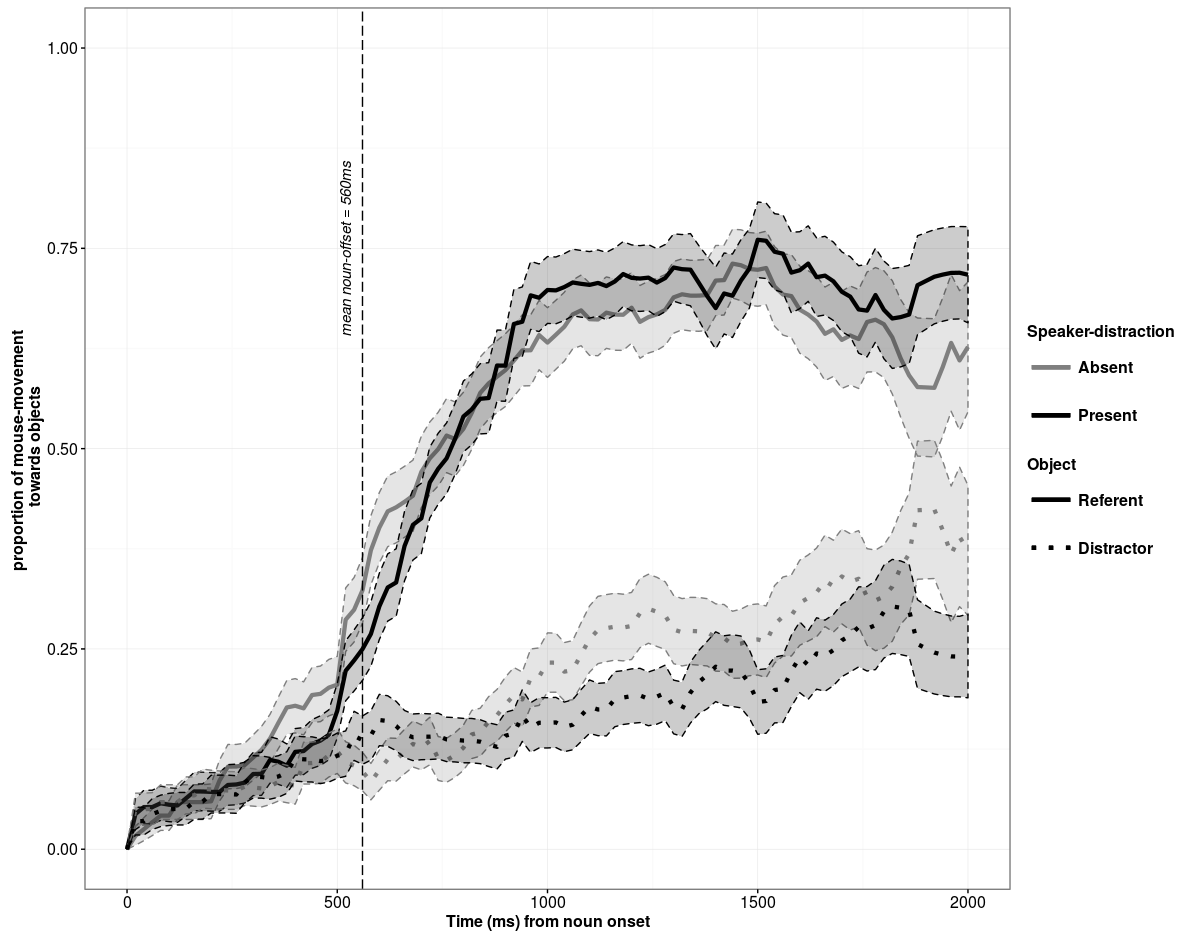
\includegraphics[scale=.5]{mflu.png}
  \caption{Mean proportion of cumulative distance traveled toward each object (referent or distractor) in fluent conditions split by presence of speaker distraction, from referent onset to 2000ms post-onset. Proportions calculated out of total cumulative distance moved the mouse from referent-onset until that time bin. Shaded areas represent $\pm 1$ standard error of the mean.}
  \label{fig:mflu}
\end{figure}





\begin{figure}
  \centering
	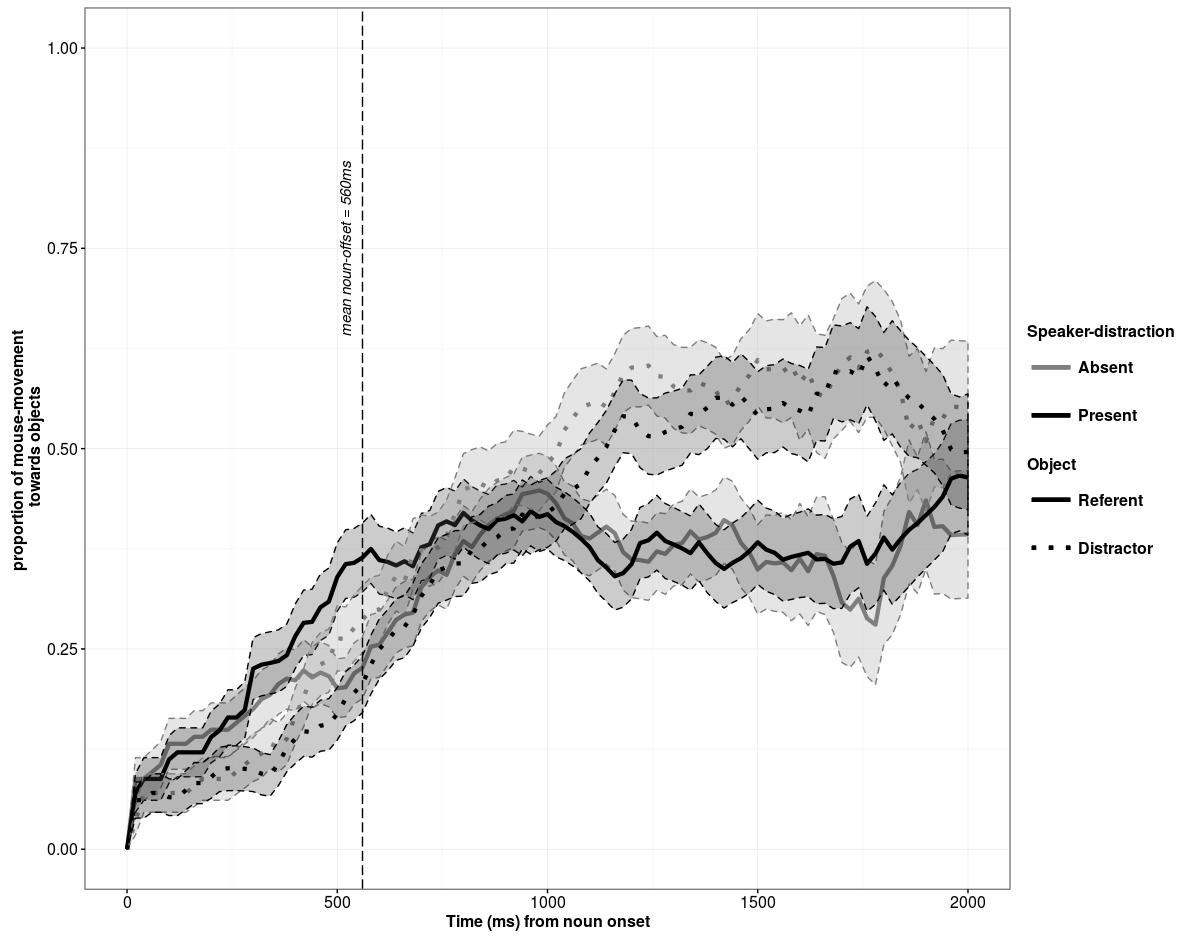
\includegraphics[scale=.5]{mdisfl.png}
  \caption{Mean proportion of cumulative distance traveled toward each object (referent or distractor) in disfluent conditions split by presence of speaker distraction, from referent onset to 2000ms post-onset. Proportions calculated out of total cumulative distance moved the mouse from referent-onset until that time bin. Shaded areas represent $\pm 1$ standard error of the mean.}
  \label{fig:mdis}
\end{figure}


\begin{figure}
  \centering
	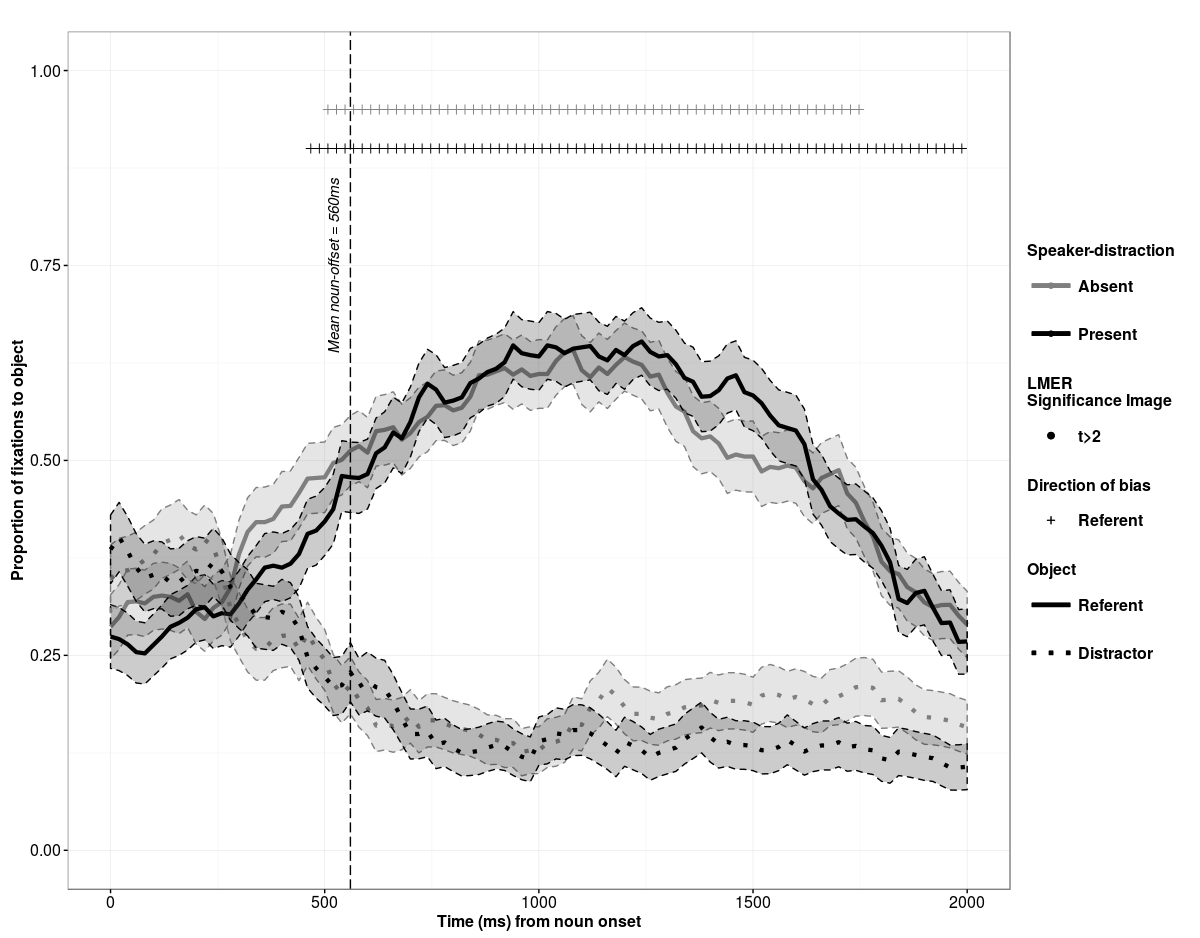
\includegraphics[scale=.5]{fluent.png}
  \caption{Mean proportion of fixations to either object (referent and distractor) for fluent utterances split by presence of speaker distraction, calculated out of the total sum of fixations for each 20ms time bin from referent-onset to 2000ms post-onset. Shaded areas represent $\pm 1$ standard error of the mean. Time bins in which a bias towards either the referent or distractor was evident are highlighted with respect to condition and direction of bias (assessed by a mixed effect model estimating the empirical logit of fixations to either object in a given condition, with main effect of object and by-subject and by-item random intercepts and random slopes of object.}
  \label{fig:flueye}
\end{figure}

\begin{figure}
  \centering
	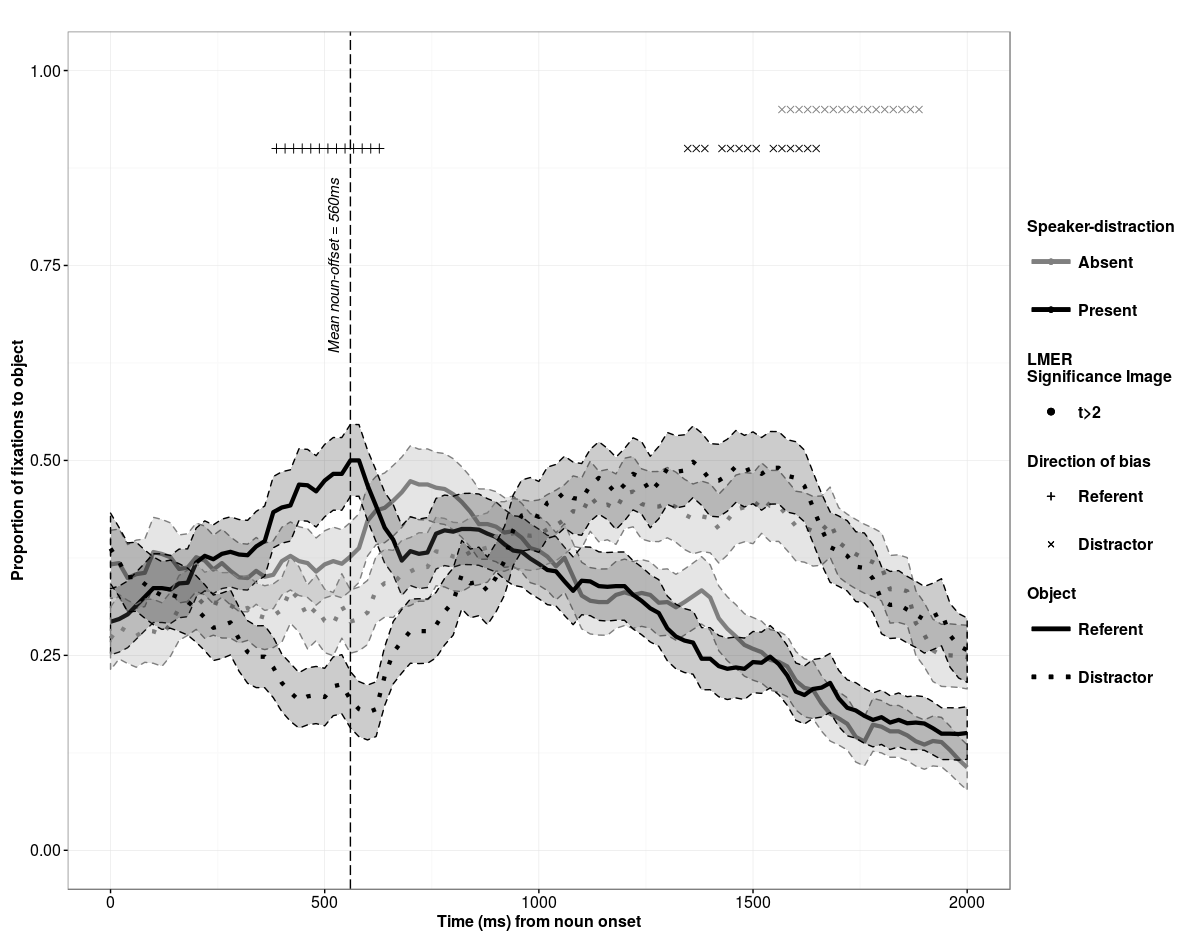
\includegraphics[scale=.5]{disfluent.png}
  \caption{Mean proportion of fixations to either object (referent and distractor) for disfluent utterances split by presence of speaker distraction, calculated out of the total sum of fixations for each 20ms time bin from referent-onset to 2000ms post-onset. Shaded areas represent $\pm 1$ standard error of the mean. Time bins in which a bias towards either the referent or distractor was evident are highlighted with respect to condition and direction of bias (assessed by a mixed effect model estimating the empirical logit of fixations to either object in a given condition, with main effect of object and by-subject and by-item random intercepts and random slopes of object.}
  \label{fig:diseye}
\end{figure}



\end{document}